\begin{enumerate}[label=\thesubsection.\arabic*.,ref=\thesubsection.\theenumi]
\numberwithin{equation}{enumi}
\item List the different kinds of damping for a second order system defined by 
\begin{align}
\label{eq:ee18btech11012_second}
H(s)=\frac{\omega^2}{s^2+2\zeta\omega+\omega^2}
\end{align}
where $\omega$ is  the natural   frequency  and $ \zeta $  is the  damping factor.
%
\\
\solution The details are available in Table \ref{table:ee18btech11012}
\begin{table}[!ht]
\centering
\begin{enumerate}[label=\thesubsection.\arabic*.,ref=\thesubsection.\theenumi]
\numberwithin{equation}{enumi}
\item List the different kinds of damping for a second order system defined by 
\begin{align}
\label{eq:ee18btech11012_second}
H(s)=\frac{\omega^2}{s^2+2\zeta\omega+\omega^2}
\end{align}
where $\omega$ is  the natural   frequency  and $ \zeta $  is the  damping factor.
%
\\
\solution The details are available in Table \ref{table:ee18btech11012}
\begin{table}[!ht]
\centering
\begin{enumerate}[label=\thesubsection.\arabic*.,ref=\thesubsection.\theenumi]
\numberwithin{equation}{enumi}
\item List the different kinds of damping for a second order system defined by 
\begin{align}
\label{eq:ee18btech11012_second}
H(s)=\frac{\omega^2}{s^2+2\zeta\omega+\omega^2}
\end{align}
where $\omega$ is  the natural   frequency  and $ \zeta $  is the  damping factor.
%
\\
\solution The details are available in Table \ref{table:ee18btech11012}
\begin{table}[!ht]
\centering
\begin{enumerate}[label=\thesubsection.\arabic*.,ref=\thesubsection.\theenumi]
\numberwithin{equation}{enumi}
\item List the different kinds of damping for a second order system defined by 
\begin{align}
\label{eq:ee18btech11012_second}
H(s)=\frac{\omega^2}{s^2+2\zeta\omega+\omega^2}
\end{align}
where $\omega$ is  the natural   frequency  and $ \zeta $  is the  damping factor.
%
\\
\solution The details are available in Table \ref{table:ee18btech11012}
\begin{table}[!ht]
\centering
\input{./tables/ee18btech11012.tex}
\caption{}
\label{table:ee18btech11012}
\end{table}

\item Classify the following second-order systems according to damping.
\label{prob:ee18btech11012_damp}
\begin{enumerate}
\item $H(s) = \frac{15}{{s^2+5s+15}}$ 
\item $H(s) = \frac{25}{{s^2+10s+25}}$
\item $H(s) =\frac{35}{{s^2+18s+35}}$ 
\end{enumerate}
\solution For 
\begin{align}
H(s) &= \frac{25}{{s^2+10s+25}},
\\
     \omega^2 &= 25,   2\zeta\omega =10\\
\implies  \omega &=1,  {\zeta} = 1
\end{align}
and the system is critically damped.  Similarly, the damping factors for other systems in Problem \ref{prob:ee18btech11012_damp} are calculated and listed in Table \ref{table:ee18btech11012_damp}
%
\begin{table}[!ht]
\centering
\input{./tables/ee18btech11012_damp.tex}
\caption{}
\label{table:ee18btech11012_damp}
\end{table}

\item By choosing an appropriate input, illustrate the effect of damping using a Python code to sketch the response.  
\end{enumerate}

\caption{}
\label{table:ee18btech11012}
\end{table}

\item Classify the following second-order systems according to damping.
\label{prob:ee18btech11012_damp}
\begin{enumerate}
\item $H(s) = \frac{15}{{s^2+5s+15}}$ 
\item $H(s) = \frac{25}{{s^2+10s+25}}$
\item $H(s) =\frac{35}{{s^2+18s+35}}$ 
\end{enumerate}
\solution For 
\begin{align}
H(s) &= \frac{25}{{s^2+10s+25}},
\\
     \omega^2 &= 25,   2\zeta\omega =10\\
\implies  \omega &=1,  {\zeta} = 1
\end{align}
and the system is critically damped.  Similarly, the damping factors for other systems in Problem \ref{prob:ee18btech11012_damp} are calculated and listed in Table \ref{table:ee18btech11012_damp}
%
\begin{table}[!ht]
\centering
\input{./tables/ee18btech11012_damp.tex}
\caption{}
\label{table:ee18btech11012_damp}
\end{table}

\item By choosing an appropriate input, illustrate the effect of damping using a Python code to sketch the response.  
\end{enumerate}

\caption{}
\label{table:ee18btech11012}
\end{table}

\item Classify the following second-order systems according to damping.
\label{prob:ee18btech11012_damp}
\begin{enumerate}
\item $H(s) = \frac{15}{{s^2+5s+15}}$ 
\item $H(s) = \frac{25}{{s^2+10s+25}}$
\item $H(s) =\frac{35}{{s^2+18s+35}}$ 
\end{enumerate}
\solution For 
\begin{align}
H(s) &= \frac{25}{{s^2+10s+25}},
\\
     \omega^2 &= 25,   2\zeta\omega =10\\
\implies  \omega &=1,  {\zeta} = 1
\end{align}
and the system is critically damped.  Similarly, the damping factors for other systems in Problem \ref{prob:ee18btech11012_damp} are calculated and listed in Table \ref{table:ee18btech11012_damp}
%
\begin{table}[!ht]
\centering
\input{./tables/ee18btech11012_damp.tex}
\caption{}
\label{table:ee18btech11012_damp}
\end{table}

\item By choosing an appropriate input, illustrate the effect of damping using a Python code to sketch the response.  
\end{enumerate}

\caption{}
\label{table:ee18btech11012}
\end{table}

\item Classify the following second-order systems according to damping.
\label{prob:ee18btech11012_damp}
\begin{enumerate}
\item $H(s) = \frac{15}{{s^2+5s+15}}$ 
\item $H(s) = \frac{25}{{s^2+10s+25}}$
\item $H(s) =\frac{35}{{s^2+18s+35}}$ 
\end{enumerate}
\solution For 
\begin{align}
H(s) &= \frac{25}{{s^2+10s+25}},
\\
     \omega^2 &= 25,   2\zeta\omega =10\\
\implies  \omega &=1,  {\zeta} = 1
\end{align}
and the system is critically damped.  Similarly, the damping factors for other systems in Problem \ref{prob:ee18btech11012_damp} are calculated and listed in Table \ref{table:ee18btech11012_damp}
%
\begin{table}[!ht]
\centering
\input{./tables/ee18btech11012_damp.tex}
\caption{}
\label{table:ee18btech11012_damp}
\end{table}

\item Find the step response of each $H(s)$ in Table \ref{table:ee18btech11012_damp}.
\\
\solution 
\begin{enumerate}
\item For 
\begin{align}
 H(s)=\frac{15}{s^2+5s+15},
\end{align}
%
the step response is
\begin{equation}
y(t)=25te^{-5t}u(t)
\label{eq:ee18btech11012_over}
\end{equation}
\item For 
%
\begin{align}
H(s)=\frac{25}{s^2+10s+25},
\end{align}
%
the step response is
\begin{equation}
y(t)=\frac{30}{\sqrt{35}}e^{\frac{-5t}{2}}\sin\brak{\frac{\sqrt{35}}{2}t}u(t)
\label{eq:ee18btech11012_critical}
\end{equation}
\item  For 

\begin{align}
H(s)=\frac{35}{s^2+18s+35},
\end{align}
the step response is
\begin{equation}
    y(t)=\frac{35}{2\sqrt{46}}\sbrak{e^{(-9+\sqrt{46})t}-e^{(-9-\sqrt{46})t}}u(t)
\label{eq:ee18btech11012_under}
\end{equation}
\end{enumerate}
\item Illustrate the effect of damping by plotting the step responses in \eqref{eq:ee18btech11012_over}-\eqref{eq:ee18btech11012_under}
\\
\solution The following code
\begin{lstlisting}
codes/ee18btech11012.py
\end{lstlisting}
%
plots the desired graphs in
Fig.     \ref{fig:ee18btech11012}. 
%
\begin{figure}[ht!]
    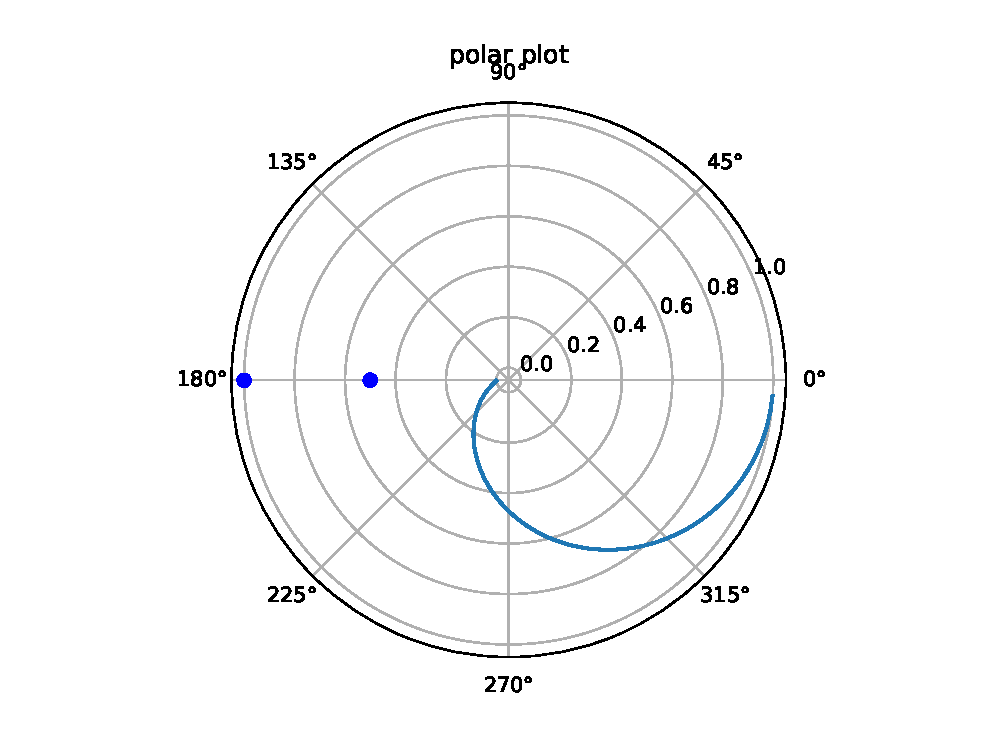
\includegraphics[width=\columnwidth]{./figs/ee18btech11012.eps}
    \caption{}
    \label{fig:ee18btech11012}
\end{figure}

\end{enumerate}
